\ifx\wholebook\relax \else

\documentclass[b5paper]{article}
\usepackage[nomarginpar
  %, margin=.5in
]{geometry}

\addtolength{\oddsidemargin}{-0.05in}
\addtolength{\evensidemargin}{-0.05in}
\addtolength{\textwidth}{0.1in}

\usepackage[en]{../../../prelude}

\setcounter{page}{1}

\begin{document}

\title{List}

\author{Xinyu~LIU
\thanks{{\bfseries Xinyu LIU} \newline
  Email: liuxinyu95@gmail.com \newline}
  }

\maketitle
\fi

\markboth{List}{Elementary Algorithms}

\ifx\wholebook\relax
\chapter{List}
\numberwithin{Exercise}{chapter}
\fi

\section{Introduction}
\label{introduction}

List and array are the preliminary build blocks to create complex data structure. Both can hold multiple elements as a container. Array is trivially implemented as a range of consecutive cells indexed by a number. The number is called address or position. Array is typically bounded. Its size need be determined before using. While list increases on-demand to hold additional elements. One can traverse a list one by one from head to tail. Particularly in functional settings, the list related algorithms play critical roles to control the computation and logic structure\footnote{In low level, lambda calculus plays the most critical role as one of the computation model equivalent to Turing machine\cite{mittype}, \cite{unplugged}.}. Readers already familiar with map, filter, fold algorithms are safe to skip this chapter, and directly start from chapter 2.

\section{Definition}
\index{List!definition}

List, also known as singly linked-list is a data structure recursively defined as below:

\begin{itemize}
\item A {\em list} is either empty, denoted as $\nil$ or NIL;
\item Or contains an element and liked with a {\em list}.
\end{itemize}

Figure \ref{fig:list-example} shows a list of nodes. Each node contains two part, an element called key, and a reference to the sub-list called next. The sub-list reference in the last node is empty, marked as `NIL'.

\begin{figure}[htbp]
  \centering
    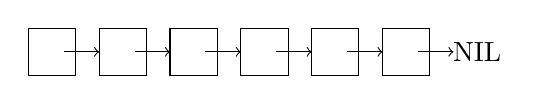
\begin{tikzpicture}[scale=3]
    \foreach \x in {-2, -1.7, ..., -0.4} {
      \draw (\x cm, 1cm) +(-0.1, -0.1) rectangle ++(0.1, 0.1);
      \draw[->] (\x cm, 1cm) +(0.05, 0) -- +(0.2, 0);
    }
    \draw (-0.2cm, 1cm) node {NIL};
    \end{tikzpicture}
  \caption{A list of nodes}
  \label{fig:list-example}
\end{figure}

Every node links to the next one or NIL. Linked-list is often defined through compound structure\footnote{In most cases, the data stored in list have the same type. However, there is also heterogeneous list, like the list in Lisp for example.}, for example:

\lstset{frame=single}
\begin{lstlisting}[language=Bourbaki]
struct List<A> {
    A key
    List<A> next
}
\end{lstlisting}

\index{List!empty} \index{List!empty testing}
It needs more clarification for the empty list. Many traditional environments support {\em null} concept. There are two different ways to represent empty list. One is to use null (or NIL) directly; the other is to construct a list, but put nothing as \texttt{[]}. From implementation perspective, null need not allocate any memory, while \texttt{[]} does. In this book, we use $\varnothing$ to represent generic empty list, set, or container.

\subsection{Access}
\index{List!head} \index{List!tail}
\index{List!Construction} \index{List!cons}
Given a none empty list $L$, we need define two functions to access its first element, and the rest sub-list. They are often called $first(L), rest(L)$ or $head(L), tail(L)$\footnote{They are named as \texttt{car} and \texttt{cdr} in Lisp due to the design of machine registers\cite{SICP}.}. On the other hand, we can construct a list from an element $x$ and another list $xs$ (can be empty), denoted as $x : xs$. It is also called the \texttt{cons} operation. We have the following equations hold:

\be
\begin{cases}
head(x:xs) & = x \\
tail(x:xs) & = xs
\end{cases}
\ee

For a none empty list $X$, we will also use $x_1$ for the first element, and use $X'$ for the rest sub-list. For example, when $X = [x_1, x_2, x_3, ...]$, then $X' = [x_2, x_3, ...]$.

\begin{Exercise}
\Question{For list of type $A$, suppose we can test if any two elements $x, y \in A$ are equal, define an algorithm to test if two lists are identical.}
\end{Exercise}

\section{Basic operations}
\index{List!length}
From the definition, we can count the length recursively: for empty list, the length is zero, otherwise, it is the length of the sub-list plus one.

\be
\begin{array}{rcl}
length(\nil) & = & 0 \\
length(L) & = & 1 + length(L')
\end{array}
\ee

In order to count the length, this algorithm traverses all the elements from head to end, hence it is bound to $O(n)$ time, where $n$ is the number of elements. To avoid repeatedly counting, we can also persist the length in a variable, and update it when mutate (add or delete) the list. Below is the iterative way to count length:

\begin{algorithmic}[1]
\Function{Length}{L}
  \State $n \gets 0$
  \While{$L \neq $ NIL}
    \State $n \gets n + 1$
    \State $L \gets $ \Call{Next}{$L$}
  \EndWhile
  \State \Return $n$
\EndFunction
\end{algorithmic}

We will also use notion $|L|$ for the length of list $L$ when the context is clear.

\subsection{index}
\index{List!index} \index{List!get at}
Different from array, which supports random access an element at position $i$ in constant time, we need traverse the list $i$ steps to access the target element.

\be
getAt(i,\ x:xs) = \begin{cases}
  i = 0: & x \\
  i \neq 0: & getAt(i - 1, xs) \\
\end{cases}
\ee

In order to get the $i$-th element from a none empty list:
\begin{itemize}
\item if $i$ is 0, the result is the first element;
\item Otherwise, the result is the $(i-1)$-th element in the sub-list.
\end{itemize}

We intend to leave the empty list not handled. The behavior when pass $\nil$ is undefined. As such, the out of bound case also leads to undefined behavior. If $i > |L|$ exceeds the length, we end up the edge case to access the $(i-|L|)$-th element of the empty list. On the other hand, if $i < 0$, minus it by one makes it even farther away from 0. We finally end up with the same situation that the index is negative, while the list is empty.

This algorithm is bound to $O(i)$ time as it advances the list $i$ steps. Below is the corresponding imperative implementation:

\begin{algorithmic}[1]
\Function{Get-At}{$i, L$}
  \While{$i \neq 0$}
    \State $L \gets $ \Call{Next}{$L$}  \Comment{Raise error when $L$ = NIL}
    \State $i \gets i - 1$
  \EndWhile
  \State \Return \Call{First}{$L$}
\EndFunction
\end{algorithmic}

\begin{Exercise}
\Question{In the iterative \textproc{Get-At}($i, L$) algorithm, what is the behavior when $L$ is empty? what is the behavior when $i$ is out of the bound or negative?}
\end{Exercise}

\subsection{Last}
\index{List!last} \index{List!init}
There is a pair of symmetric operations to `first/rest'. They are called `last/init'. For a none empty list $X = [x_1, x_2, ..., x_n]$, function $last$ returns the last element $x_n$, while $init$ returns the sub-list of $[x_1, x_2, ..., x_{n-1}]$. Although they are symmetric pairs left to right, `last/init' need linear time, because we need traverse the whole list to tail.


When access the last element of list $X$:
\begin{itemize}
\item If the $X$ contains only one element as $[x_1]$, then $x_1$ is the last one;
\item Otherwise, the result is the last element of the sub-list $X'$.
\end{itemize}

\be
\begin{array}{rcl}
last([x]) & = & x \\
last(x:xs) & = & last(xs) \\
\end{array}
\ee

Similarly, when extract the sub-list of $X$ contains all elements without the last one:

\begin{itemize}
\item If $X$ is a singleton $[x_1]$, the result is empty $[\ ]$;
\item Otherwise, we recursively get the initial sub-list for $X'$, then prepend $x_1$ to it as the result.
\end{itemize}

\be
\begin{array}{rcl}
init([x]) & = & [\ ] \\
init(x:xs) & = & x : init(xs) \\
\end{array}
\ee

We leave the empty list not handled for both operations. The behavior is undefined if pass $\nil$ in. Below are the iterative implementation:

\begin{algorithmic}[1]
\Function{Last}{$L$}
  \State $x \gets $ NIL
  \While{$L \neq$ NIL}
    \State $x \gets $ \Call{First}{$L$}
    \State $L \gets $ \Call{Rest}{$L$}
  \EndWhile
  \State \Return $x$
\EndFunction
\Statex
\Function{Init}{$L$}
  \State $L' \gets $ NIL
  \While{\Call{Rest}{$L$} $\neq$ NIL} \Comment{Raise error when $L$ is NIL}
    \State $L' \gets$ \textproc{Cons}(\Call{First}{$L$}, $L'$)
    \State $L \gets $ \Call{Rest}{$L$}
  \EndWhile
  \State \Return \Call{Reverse}{$L'$}
\EndFunction
\end{algorithmic}

As advancing towards the tail, this algorithm accumulates the `init' result through `cons'. However, such result is in the reversed order. We need apply reverse (defined in section \ref{sec:reverse}) again to return the correct result. There is a question to ask if we can use `append' instead of `cons' in the exercise.

\subsection{Reverse index}
\index{List!Reverse index} \index{List!rindex}
$last$ is a special case of reverse index. The generic case is to find the last $i$-th element of a given list. The naive implementation takes two rounds of traverse: Determine the length $n$ through the first round; then access the $(n - i - 1)$-th element through the second round:

\be
  lastAt(i, L) = getAt(|L| - i - 1, L)
\ee

There actually exists better solution. The idea is to keep two pointers $p_1, p_2$ with the distance $i$ between them. The equation $rest^i(p_2) = p_1$ holds, where $rest^i(p_2)$ means repleatedly apply $rest()$ function $i$ times. When succeed $p_2$ by $i$ steps gets $p_1$. We start by pointing $p_2$ to the list head, and advance both pointers in parallel till $p_1$ arrives at tail. At that time point, $p_2$ exactly points to the $i$-th element from right. Figure \ref{fig:list-rindex} shows this idea. As $p_1, p_2$ form a window, this method is also called `sliding window' solution.

\begin{figure}[htbp]
  \centering
  \subcaptionbox{$p_2$ starts from the head, behind $p_1$ in $i$ steps.}{\includegraphics[scale=0.8]{img/list-rindex.ps}} \\
  \subcaptionbox{When $p_1$ reaches the tail, $p_2$ points to the $i$-th element from right.}{\includegraphics[scale=0.8]{img/list-rindex-2.ps}}
  \caption{Sliding window formed by two pointers}
  \label{fig:list-rindex}
\end{figure}

\begin{algorithmic}[1]
\Function{Last-At}{$i, L$}
  \State $p \gets L$
  \While{$i > 0$}
    \State $L \gets $ \Call{Rest}{$L$} \Comment{Raise error if out of bound}
    \State $i \gets i - 1$
  \EndWhile
  \While{\Call{Rest}{$L$} $\neq$ NIL}
    \State $L \gets$ \Call{Rest}{$L$}
    \State $p \gets$ \Call{Rest}{$p$}
  \EndWhile
  \State \Return \Call{First}{$p$}
\EndFunction
\end{algorithmic}

The functional implementation need special consideration as we cannot update pointers directly. Instead, we advance two lists $X = [x_1, x_2, ..., x_n]$ and $Y = [x_i, x_{i+1}, ..., x_n]$ simultaneously, where $Y$ is the sub-list without the first $i - 1$ elements.

\begin{itemize}
\item If $Y$ is a singleton list, i.e. $[x_n]$, then the last $i$-th element is the head of $X$;
\item Otherwise, we drop the first element from both $X$ and $Y$, then recursively check $X'$ and $Y'$.
\end{itemize}

\be
lastAt(i, X) = slide(X, drop(i, X))
\ee

where function $slide(X, Y)$ drops the heads for both lists:

\be
\begin{array}{rcl}
slide(x:xs,\ [y]) & = & x \\
slide(x:xs,\ y:ys) & = & slide(xs, ys) \\
\end{array}
\ee

Function $drop(m, X)$ discards the first $m$ elements from list $X$. It can be implemented by advancing $X$ by $m$ steps:

\be
\begin{array}{rcl}
drop(0,\ X) & = & X \\
drop(m,\ \nil) & = & \nil \\
drop(m,\ x:xs) & = & drop(m - 1, xs) \\
\end{array}
\ee

\begin{Exercise}
\Question{In the \textproc{Init} algorithm, can we use \textproc{Append}($L'$, \textproc{First}($L$)) instead of `cons'?}
\Question{How to handle empty list or out of bound index error in \textproc{Last-At} algorithm?}
\end{Exercise}

\subsection{Mutate}
\index{List!mutate}
Mutate operations include append, insert, update, and delete. Some functional environments actually implement mutate by creating a new list, while the original one is persisted for later reuse, or released at sometime (chapter 2 in \cite{okasaki-book}).

\subsubsection{Append}
\index{List!append}
Append is the symmetric operation of $cons$, it adds element on the tail instead of head. Because of this, it is also called `snoc'. For linked-list, it means we need traverse to the tail, hence it takes $O(n)$ time, where $n$ is the length. To avoid repeatedly traverse, we can record the tail reference as a variable, and keep updating it upon changes.

\be
\begin{array}{rcl}
append(\nil, x) & = & [x] \\
append(y:ys, x) & = & y : append(ys, x) \\
\end{array}
\ee

\begin{itemize}
\item If append $x$ to the empty list, the result is $[x]$;
\item Otherwise, we firstly recursive append $x$ to the rest sub-list, then prepend the original head to form the result.
\end{itemize}

The corresponding iterative implementation is as the following:

\begin{algorithmic}[1]
\Function{Append}{$L, x$}
  \If{$L = $ NIL}
    \State \Return \Call{Cons}{$x$, NIL}
  \EndIf
  \State $H \gets L$ \Comment{save the head}
  \While{\Call{Rest}{$L$} $\neq$ NIL}
    \State $L \gets$ \Call{Rest}{$L$}
  \EndWhile
  \State \Call{Rest}{$L$} $\gets$ \Call{Cons}{$x$, NIL}
  \State \Return $H$
\EndFunction
\end{algorithmic}

Update the \textproc{Rest} is typically implemented by setting the \texttt{next} reference field as shown in below example program.

\begin{lstlisting}[language=Bourbaki]
List<A> append(List<A> xs, T x) {
    if (xs == null) {
        return cons(x, null)
    }
    List<A> head = xs
    while (xs.next != null) {
        xs = xs.next
    }
    xs.next = cons(x, null)
    return head
}
\end{lstlisting}

\begin{Exercise}
\Question{Add a `tail' field in list definition, optimize the append algorithm to constant time.}
\Question{With the additional `tail' field, when need we update the tail variable? How does it affect the performance?}
\end{Exercise}

\subsubsection{Set value}
\index{List!set at}
Similar to $getAt$, we need advance to the target position, then change the element there. To define function $setAt(i, x, L)$:

\begin{itemize}
\item If $i = 0$, it means we are changing the first element, the result is $x : L'$;
\item Otherwise, we need recursively set the value at position $i-1$ for the sub-list $L'$.
\end{itemize}

\be
\begin{array}{rcl}
setAt(0, x,\ y:ys) & = & x : ys \\
setAt(i, x,\ y:ys) & = & y : setAt(i - 1, x, ys) \\
\end{array}
\ee

This algorithm is bound to $O(i)$ time, where $i$ is the position to update.

\begin{Exercise}
\Question{Handle the empty list and out of bound error for $setAt$.}
\end{Exercise}

\subsubsection{insert}
\index{List!insert} \index{List!insert at}
There are two different cases about insertion. One is to insert an element at a given position: $insert(i, x, L)$. The algorithm is similar to $setAt$; The other is to insert an element to a sorted list, and keep the order still sorted.

To insert $x$ at position $i$, we need firstly advance $i$ steps, then construct a new sub-list with $x$ as the head, then concatenate it to the first $i$ elements.

\begin{itemize}
\item If $i = 0$, it then turns to be a `cons' operation: $x : L$;
\item Otherwise, we recursively insert $x$ to $L'$ at position $i-1$; then prepend the original head.
\end{itemize}

\be
\begin{array}{rcl}
insert(0, x,\ L) & = & x : L \\
insert(i, x,\ y:ys) & = & x : insert(i - 1, x, ys) \\
\end{array}
\ee

When $i$ exceeds the list length, we can treat it as to append $x$. We leave this as an exercise. The following is the corresponding iterative implementation:

\begin{algorithmic}[1]
\Function{Insert}{$i, x, L$}
  \If{$i = 0$}
    \State \Return \Call{Cons}{$x, L$}
  \EndIf
  \State $H \gets L$
  \State $p \gets L$
  \While{$i > 0$ and $L \neq$ NIL}
    \State $p \gets L$
    \State $L \gets $ \Call{Rest}{$L$}
    \State $i \gets i - 1$
  \EndWhile
  \State \Call{Rest}{$p$} $\gets$ \Call{Cons}{$x, L$}
  \State \Return $H$
\EndFunction
\end{algorithmic}

If the list $L = [x_1, x_2, ..., x_n]$ is sorted, i.e. for any position $1 \leq i \leq j \leq n$, then $x_i \leq x_j$ holds. Here $\leq$ is abstract ordering. It can actually mean $\geq$ for descending order, or subset relationship etc. We can design the insert algorithm to maintain the sorted order. To insert element $x$ to a sorted list $L$:

\begin{itemize}
\item If either $L$ is empty or $x$ is not greater than the first element in $L$, we prepend $x$ to $L$ and returns $x : L$;
\item Otherwise, we recursively insert $x$ to the sub-list $L'$.
\end{itemize}

\be
\begin{array}{rcl}
insert(x,\ \nil) & = & [x] \\
insert(x,\ y : ys) & = & \begin{cases}
  x \leq y : & x : y : ys \\
  otherwise : & y : insert(x, ys) \\
  \end{cases}
\end{array}
\ee

Since the algorithm need compare elements one by one, it is bound to $O(n)$ time, where $n$ is the length. Below is the corresponding iterative implementation:

\begin{algorithmic}[1]
\Function{Insert}{$x, L$}
  \If{$L = $ NIL or $x <$ \Call{First}{$L$}}
    \State \Return \Call{Cons}{$x, L$}
  \EndIf
  \State $H \gets L$
  \While{\Call{Rest}{$L$} $\neq $ NIL and \textproc{First}(\Call{Rest}{$L$}) $< x$}
    \State $L \gets $ \Call{Rest}{$L$}
  \EndWhile
  \State \Call{Rest}{$L$} $\gets$ \textproc{Cons}($x$, \Call{Rest}{$L$})
  \State \Return $H$
\EndFunction
\end{algorithmic}

\label{sec:isort}
With this linear time ordered insertion defined, we can further develop the insertion-sort algorithm. The idea is to repeatedly insert elements to the empty list. Since each insert takes liner time, the overall sort is bound to $O(n^2)$.

\be
\begin{array}{rcl}
sort(\nil) & = & \nil \\
sort(x:xs) & = & insert(x, sort(xs)) \\
\end{array}
\ee

This is a recursive algorithm. It firstly sorts the sub-list, then inserts the first element in it. We can eliminate the recursion to develop a iterative implementation. The idea is to scan the list, and one by one insert them:

\begin{algorithmic}[1]
\Function{Sort}{$L$}
  \State $L' \gets$ NIL
  \While{$L \neq$ NIL}
    \State $L' \gets$ \textproc{Insert}(\Call{First}{$L$}, $L'$)
    \State $L \gets$ \Call{Rest}{$L$}
  \EndWhile
  \State \Return $L'$
\EndFunction
\end{algorithmic}

At any time during the loop, the result is sorted. There is a major difference between the recursive and the iterative implementations. The recursive one processes the list from right, while the iterative one is from left. We'll introduce `tail-recursion' in section \ref{sec:tail-call} to eliminate this difference. Chapter 3 introduces insertion sort in detail, including performance analysis and optimization.

\begin{Exercise}
\Question{Handle the out-of-bound case in insertion, and treat it as append.}
\Question{Design the insertion algorithm for array. When insert at position $i$, all elements after $i$ need shift to the end by one.}
\Question{Implement the insertion sort only with less than ($<$) defined.}
\end{Exercise}

\subsubsection{delete}
\index{List!delete} \index{List!delete at}
Symmetric to insert, delete also has two cases. One is to delete the element at a position; the other is to look up, then delete the element of a given value. The first case is defined as $delAt(i, L)$, the second case is defined as $delete(x, L)$.

To delete the element at position $i$, we need advance $i$ steps to the target position, then by pass the element, and link the rest sub-list.
\begin{itemize}
\item If $L$ is empty, then the result is empty too;
\item If $i = 0$, we are deleting the head, the result is $L'$;
\item Otherwise, recursively delete the $(i-1)$-th element from $L'$, then prepend the original head as the result.
\end{itemize}

\be
\begin{array}{rcl}
delAt(i,\ \nil) & = & \nil \\
delAt(0,\ x:xs) & = & xs \\
delAt(i,\ x:xs) & = & x : delAt(i - 1, xs) \\
\end{array}
\ee

This algorithm is bound to $O(i)$ as we need advance $i$ steps to perform deleting. Below is the iterative implementation:

\begin{algorithmic}[1]
\Function{Del-At}{$i, L$}
  \State $S \gets$ \Call{Cons}{$\perp, L$} \Comment{A sentinel node}
  \State $p \gets S$
  \While{$i > 0$ and $L \neq$ NIL}
    \State $i \gets i - 1$
    \State $p \gets L$
    \State $L \gets $ \Call{Rest}{$L$}
  \EndWhile
  \If{$L \neq$ NIL}
    \State \Call{Rest}{$p$} $\gets$ \Call{Rest}{$L$}
  \EndIf
  \State \Return \Call{Rest}{$S$}
\EndFunction
\end{algorithmic}

To simplify the implementation, we introduce a sentinel node $S$, it contains a special value $\perp$, and its next reference points to $L$. With $S$, we are save to cut-off any node in $L$ even for the first one. Finally, we return the list after $S$ as the result, and $S$ itself can be discarded.

For the `find and delete' case, there are two options. We can either find and delete the first occurrence of a value; or remove all the occurrences. The later is more generic, we leave it as an exercise. When delete $x$ from list $L$:

\begin{itemize}
\item If the list is empty, the result is $\nil$;
\item Otherwise, we compare the head and $x$, if they are equal, then the result is $L'$;
\item If the head does not equal to $x$, we keep the head, and recursively delete $x$ in $L'$.
\end{itemize}

\be
\begin{array}{rcl}
delete(x,\ \nil) & = & \nil \\
delete(x,\ y:ys) & = & \begin{cases}
  x = y : & delete(x, ys) \\
  x \neq y : & y : delete(x, ys) \\
  \end{cases} \\
\end{array}
\ee

This algorithm is bound to $O(n)$ time, where $n$ is the length, as it need scan the list to find the target element. For the iterative implementation, we also introduce a sentinel node to simplify the logic:

\begin{algorithmic}[1]
\Function{Delete}{$x, L$}
  \State $S \gets$ \Call{Cons}{$\perp, L$}
  \State $p \gets$ L
  \While{$L \neq$ NIL and \Call{First}{$L$} $\neq x$}
    \State $p \gets L$
    \State $L \gets$ \Call{Rest}{$L$}
  \EndWhile
  \If{$L \neq$ NIL}
    \State \Call{Rest}{$p$} $\gets$ \Call{Rest}{$L$}
  \EndIf
  \State \Return \Call{Rest}{$S$}
\EndFunction
\end{algorithmic}

\begin{Exercise}
\Question{Design the algorithm to find and delete all occurrences of a given value.}
\Question{Design the delete algorithm for array, all elements after the delete position need shift to front by one.}
\end{Exercise}

\subsubsection{concatenate}
\label{concat} \index{List!concat}
Append is a special case for concatenation. Append only adds one element, while concatenation adds multiple ones. However, the performance would be quadratic if repeatedly appending as below:

\be
\begin{array}{rcl}
X \doubleplus \nil & = & X \\
X \doubleplus (y:ys) & = & append(X, y) \doubleplus ys \\
\end{array}
\ee

In this implementation when concatenate $X$ and $Y$, each append operation traverses to the tail, and we do this for $|Y|$ times. the total time is bound to $O(|X| + (|X| + 1) + ... + (|X| + |Y|)) = O(|X||Y| + |Y|^2)$. Consider the link (cons) operation is fast (constant time), we can traverse to the tail of $X$ only once, then link $Y$ to the tail.

\begin{itemize}
\item If $X$ is empty, the result is $Y$;
\item Otherwise, we concatenate the sub-list $X'$ with $Y$, then prepend the head as the result.
\end{itemize}

We can further improve it a bit: when $Y$ is empty, we needn't traverse, but directly return $X$:

\be
\begin{array}{rcl}
\nil \doubleplus Y & = & Y \\
X \doubleplus \nil & = & X \\
(x:xs) \doubleplus Y & = & x : (xs \doubleplus Y) \\
\end{array}
\ee

The modified algorithm only traverse list $X$, then link its tail to $Y$, hence it is bound $O(|X|)$ time. In imperative settings, concatenation can be realized in constant time with the additional tail variable. We leave its implementation as exercise. Below is the iterative implementation without using the tail variable:

\begin{algorithmic}[1]
\Function{Concat}{$X, Y$}
  \If{$X = $ NIL}
    \State \Return $Y$
  \EndIf
  \If{$Y = $ NIL}
    \State \Return $X$
  \EndIf
  \State $H \gets X$
  \While{\Call{Rest}{$X$} $\neq$ NIL}
    \State $X \gets$ \Call{Rest}{$X$}
  \EndWhile
  \State \Call{Rest}{$X$} $\gets Y$
  \State \Return $H$
\EndFunction
\end{algorithmic}

\subsection{sum and product}
\index{List!sum} \index{List!product}
It is common to calculate the sum or product of a list of numbers. They have almost same structure. We will introduce how to abstract them to higher order computation in section \ref{sec:fold}.

\subsubsection{Recursive sum and product}

To calculate the sum of a list:

\begin{itemize}
\item If the list is empty, the result is zero;
\item Otherwise, the result is the first element plus the sum of the rest.
\end{itemize}

\be
\begin{array}{rcl}
sum(\nil) & = & 0 \\
sum(x:xs) & = & x + sum(xs) \\
\end{array}
\ee

We can't merely replace $+$ to $\times$ to obtain product algorithm, because it always returns zero. We need define the product of the empty list as 1.

\be
\begin{array}{rcl}
product(\nil) & = & 1 \\
product(x:xs) & = & x \cdot product(xs) \\
\end{array}
\ee

Both algorithms traverse the list, hence are bound to $O(n)$ time, where $n$ is the length.

\subsubsection{Tail call recursion}
\index{Tail call} \index{Tail recursion} \index{Tail recursive call}
\label{sec:tail-call}
Both sum and product algorithms calculate from right to left. We can change them to calculate the {\em accumulated} result from left to right. For sum, it accumulates from 0, then adds element one by one; while for product, it starts from 1, then repeatedly multiplying elements. The accumulate process can be defined as:

\begin{itemize}
\item If the list is empty, return the accumulated result;
\item Otherwise, accumulate the first element to the result, then go on accumulating.
\end{itemize}

Below are the accumulated sum and product:

\be
\begin{array}{cc}
  \begin{array}{rl}
  sum'(A,\ \nil) = & A \\
  sum'(A,\ x:xs) = & sum(x + A, xs) \\
  \end{array}
  &
  \begin{array}{rl}
  prod'(A,\ \nil) = & A \\
  prod'(A,\ x:xs) = & prod'(x \cdot A, xs) \\
  \end{array} \\
\end{array}
\ee

Given a list, we can call $sum'$ with 0, and $prod'$ with 1:

\be
sum(X) = sum'(0, X)
\quad \quad \quad
product(X) = prod'(1, X)
\ee

Or merely simplify it to Curried form:

\[
sum = sum'(0) \quad \quad \quad product = prod'(1)
\]

\index{Curried Form} \index{Currying}
Curried form was introduced by Schönfinkel (1889 - 1942) in 1924, then widely used by Haskell Curry from 1958. It is known as {\em Currying}\cite{slpj-book-1987}. For a function taking 2 parameters $f(x, y)$, when pass one argument $x$, it ends up to another function of $y$: $g(y) = f(x, y)$ or $g = f\ x$. We can further extend it to multiple variables, that $f(x, y, ..., z)$ can be Curried to a series of functions: $f, f\ x, f\ x\ y\, ...$. No matter how many variables, we can treat them as a series of Curried function, each has only one parameter: $f(x, y, ..., z) = f(x)(y)...(z) = f\ x\ y\ ...\ z$.

The accumulated sum does not only calculate the result from left to right, it needn't book keeping any context, state, or intermediate result for recursion. All such states are either passed as argument (i.e. $A$), or can be dropped (the previous element in the list). Such recursive calls are often optimized as pure loops in practice. We call this kind of function as {\em tail recursion} (or `tail call'), and the optimization to eliminate recursion is called 'tail recursion optimization'\cite{wiki-tail-call}, because the recursion happens at the tail place in the function. The performance of tail call can be greatly improved after optimization, and we can avoid the issue of stack overflow in deep recursions.

In section \ref{sec:isort} about insertion sort, we mentioned the recursive algorithm sorts elements form right. We can also optimize it to tail call:

\be
\begin{array}{rcl}
sort'(A,\ \nil) & = & A \\
sort'(A,\ x:xs) & = & sort'(insert(x, A), xs) \\
\end{array}
\ee

And the sort is defined in Curried form with $\nil$ as the start value:

\be
sort = sort'(\nil)
\ee

As a typical tail call problem, let's consider how to compute $b^n$ effectively? (refer to problem 1.16 in \cite{SICP}.) A brute-force solution is to repeatedly multiplying $b$ for $n$ times from 1. This algorithm is bound to $O(n)$:

\begin{algorithmic}[1]
\Function{Pow}{$b, n$}
  \State $x \gets 1$
  \Loop{ $n$ times}
    \State $x \gets x b$
  \EndLoop
  \State \Return $x$
\EndFunction
\end{algorithmic}

Actually, the solution can be greatly improved. When compute $b^8$, after the first 2 loops, we get $x = b^2$. At this stage, we
needn't multiply $x$ with $b$ to get $b^3$, but directly compute $x^2$, which gives $b^4$. If do this again, we get $(b^4)^2 = b^8$. Thus we only need loop 3 times, but not 8 times.

Based on this idea, if $n = 2^m$ for some none negative integer $m$, we can design below algorithm to compute $b^n$:

\[
\begin{array}{rcl}
b^1 & = & b \\
b^n & = & (b^{\frac{n}{2}})^2 \\
\end{array}
\]

We next extend this divide and conquer method for any none negative integer $n$:

\begin{itemize}
\item If $n = 0$, define $b^0 = 1$;
\item If $n$ is even, we halve $n$, to compute $b^{\frac{n}{2}}$. Then square it;
\item Otherwise $n$ is odd. Since $n-1$ is even, we recursively compute $b^{n-1}$, the multiply $b$ atop it.
\end{itemize}

\be
\begin{array}{rcl}
b^0 & = & 1 \\
b^n & = & \begin{cases}
2 | n : & (b^{\frac{n}{2}})^2 \\
otherwise : & b \cdot b^{n-1} \\
\end{cases}
\end{array}
\ee

However, the 2nd clause blocks us to turn it tail recursive. Alternatively, we can square the base number, and halve the exponent.

\be
\begin{array}{rcl}
b^0 & = & 1 \\
b^n & = & \begin{cases}
2 | n : & (b^2)^{\frac{n}{2}} \\
otherwise : & b \cdot b^{n-1} \\
\end{cases}
\end{array}
\ee

With this change, we can develop a tail recursive algorithm to compute $b^n = pow(b, n, 1)$.

\be
\begin{array}{rcl}
pow(b, 0, A) & = & A \\
pow(b, n, A) & = & \begin{cases}
  2 | n : & pow(b^2, \dfrac{n}{2}, A) \\
  otherwise: & pow(b, n - 1, b \cdot A) \\
\end{cases}
\end{array}
\ee

Compare to the brute-force implementation, this one improves to $O(\lg n)$ time. Actually, we can improve it further. If represent $n$ in binary format $n = (a_ma_{m-1}...a_1a_0)_2$, we clearly know that the computation for $b^{2^i}$ is necessary if $a_i = 1$. This is quite similar to the idea of Binomial heap (section \autoref{sec:binomial-heap}). We can multiplying all of them for bits of 1.

For example, when compute $b^{11}$, as $11 = (1011)_2 = 2^3 + 2 +1$, thus $b^{11} = b^{2^3} \times b^2 \times b$. We get the result by these steps:

\begin{enumerate}
\item calculate $b^1$, which is $b$;
\item Square to $b^2$ from the previous result;
\item Square again to $b^{2^2}$ from step 2;
\item Square to $b^{2^3}$ from step 3.
\end{enumerate}

Finally, we multiply the result of step 1, 2, and 4 to get $b^{11}$. Summarize this idea, we improve the algorithm as below.

\be
\begin{array}{rcl}
pow(b, 0, A) & = & A \\
pow(b, n, A) & = & \begin{cases}
  2 | n : & pow(b^2, \dfrac{n}{2}, A) \\
  otherwise: & pow(b^2, \lfloor \dfrac{n}{2} \rfloor, b \cdot A) \\
  \end{cases}
\end{array}
\ee

This algorithm essentially shifts $n$ to right 1 bit each time (divide $n$ by 2). If the LSB (Least Significant Bit, the lowest) is 0, $n$ is even. It squares the base and keeps the accumulator $A$ unchanged; If the LSB is 1, $n$ is odd. It squares the base and accumulates it to $A$; When $n$ is zero, we exhaust all bits, $A$ is the final result. At any time, the updated base number $b'$, the shifted exponent number $n'$, and the accumulator $A$ satisfy the invariant $b^n = A \cdot (b')^{n'}$.

Compare to previous implementation, which minus by one for odd $n$, this algorithm halves $n$ every time. It exactly runs $m$ rounds, where $m$ is the number of bits. We leave the imperative implementation as exercise.

Back to the sum and product. The iterative implementation applies plus and multiply while traversing:

\begin{algorithmic}[1]
\Function{Sum}{$L$}
  \State $s \gets 0$
  \While{$L \neq$ NIL}
    \State $s \gets s +$ \Call{First}{$L$}
    \State $L \gets$ \Call{Rest}{$L$}
  \EndWhile
  \State \Return $s$
\EndFunction
\Statex
\Function{Product}{$L$}
  \State $p \gets 1$
  \While{$L \neq$ NIL}
    \State $p \gets p \times $ \Call{First}{$L$}
    \State $L \gets$ \Call{Rest}{$L$}
  \EndWhile
  \State \Return $p$
\EndFunction
\end{algorithmic}

One interesting usage of product is to calculate factorial of $n$ as: $n! = product([1..n])$.

\subsection{maximum and minimum}
\index{List!maximum} \index{List!minimum}

For a list of comparable elements (we can define order for any two elements), there is the maximum and minimum. The algorithm structure of $max/min$ is same. For a none empty list:

\begin{itemize}
\item If there is only one element (a singleton) $[x_1]$, the result is $x_1$;
\item Otherwise, we recursively find the min/max of the sub-list, then compare it with the first element to determine the result.
\end{itemize}

\be
  \begin{array}{rcl}
  min([x]) & = & x \\
  min(x:xs) & = & \begin{cases}
    x < min(xs) : & x \\
    otherwise: & min(xs) \\
  \end{cases}
  \end{array}
\ee
and
\be
  \begin{array}{rcl}
  max([x]) & = & x \\
  max(x:xs) & = & \begin{cases}
    x > max(xs) : & x \\
    otherwise: & max(xs) \\
  \end{cases}
  \end{array}
\ee

Both process the list from right to left. We can modify them to tail recursive. It also brings us the `on-line' feature, that at any time, the accumulator is the min/max so far processed. Use $min$ for example:

\be
\begin{array}{rcl}
min'(a,\ \nil) & = & a \\
min'(a,\ x:xs) & = & \begin{cases}
  x < a : & min'(x, xs) \\
  otherwise : & min'(a, xs) \\
  \end{cases}
\end{array}
\ee

Different from $sum'/prod'$, we can't pass a fixed starting value to the tail recursive $min'/max'$, unless we use $\pm \infty$ in below Curried form:

\[
  min = min'(\infty) \quad \quad \quad max = max'(- \infty)
\]

Alternatively, we can pass the first element as the accumulator given min/max only takes none empty list:

\be
  min(x:xs) = min'(x,\ xs)
  \quad \quad \quad
  max(x:xs) = max'(x,\ xs)
\ee

The optimized tail recursive algorithm can be further changed to purely iterative implementation. We give the \textproc{Min} example, and skip \textproc{Max}.

\begin{algorithmic}[1]
\Function{Min}{$L$}
  \State $m \gets$ \Call{First}{$L$}
  \State $L \gets$ \Call{Rest}{$L$}
  \While{$L \neq$ NIL}
    \If{\Call{First}{$L$} $< m$ }
      \State $m \gets$ \Call{First}{$L$}
    \EndIf
    \State $L \gets$ \Call{Rest}{$L$}
  \EndWhile
  \State \Return $m$
\EndFunction
\end{algorithmic}

There is a way to realize the tail recursive algorithm without using accumulator explicitly. The idea is to re-use the first element as the accumulator. Every time, we compare the head with the next element; then drop the greater one for $min$, and drop the less one for $max$.

\be
\begin{array}{rcl}
min([x]) & = & x \\
min(x_1:x_2:xs) & = & \begin{cases}
  x_1 < x_2 : & min(x_1:xs) \\
  otherwise: & min(x_2:xs) \\
  \end{cases}
\end{array}
\ee

We skip the definition for $max$ as it is symmetric.

\begin{Exercise}
\Question{Change the $length$ to tail call.}
\Question{Change the insertion sort to tail call.}
\Question{Implement the $O(\lg n)$ algorithm to calculate $b^n$ by represent $n$ in binary.}
\end{Exercise}

\section{Transform}
\index{List!Transform}
From algebraic perspective, there are two types of transform: one keeps the list structure, but only change the elements; the other alter the list structure, hence the result is not isomorphic to the original list. Particularly, we call the former {\em map}.

\subsection{map and for-each}
\index{List!map}
The first example is to convert a list of numbers to their represented strings, like to change [3, 1, 2, 4, 5] to [``three'', ``one'', ``two'', ``four'', ``five'']

\be
\begin{array}{rcl}
toStr(\nil) & = & \nil \\
toStr(x:xs) & = & str(x) : toStr(xs) \\
\end{array}
\label{eq:tostr}
\ee

For the second example, consider a dictionary, which is a list of words grouped by initial letter. Like:

\begin{verbatim}
[[a, an, another, ... ],
 [bat, bath, bool, bus, ...],
 ...,
 [zero, zoo, ...]]
\end{verbatim}

Next we process a text ({\em Hamlet} for example), and augment each word with their number of occurrence, like:

\begin{verbatim}
[[(a, 1041), (an, 432), (another, 802), ... ],
 [(bat, 5), (bath, 34), (bool, 11), (bus, 0), ...],
 ...,
 [(zero 12), (zoo, 0), ...]]
\end{verbatim}

Now for every initial letter, we want to figure out which word occurs most. How to write a program to do this work? The output is a list of words, that every one has the most occurrences in the group, something like \texttt{[a, but, can, ...]}. We need develop a program that transform \textbf{a list of groups of word-number pairs} into \textbf{a list of words}.

First, we need define a function. It takes a list of word-number pairs, finds the word paired with the biggest number. Sort is overkill. What we need is a special max function $maxBy(cmp, L)$, where $cmp$ compares two elements abstractly.

\be
\begin{array}{rcl}
maxBy(cmp,\ [x]) & = & x \\
maxBy(cmp,\ x_1 : x_2 : xs) & = & \begin{cases}
  cmp(x_1, x_2) : & maxBy(cmp, x_2 : xs) \\
  otherwise : & maxBy(cmp, x_1 : xs) \\
  \end{cases}
\end{array}
\ee

For a pair $p = (a, b)$ we define two access functions:

\be
\begin{cases}
fst\ (a, b) = & a \\
snd\ (a, b) = & b \\
\end{cases}
\ee

Instead of embedded parenthesis $fst((a, b)) = a$, we omit one layer, and use a space. Generally, we treat $f\ x = f(x)$ when the context is clear. Then we can define a special compare function for word-count pairs:

\be
less(p_1, p_2) = snd(p_1) < snd(p_2)
\ee

Then pass $less$ to $maxBy$ to finalize our definition (in Curried form):

\be
max'' = maxBy(less)
\ee

With $max''()$ defined, we can develop the solution to process the whole list.

\be
\begin{array}{rcl}
solve(\nil) & = & \nil \\
solve(x:xs) & = & fst(max''(x)) : solve(xs) \\
\end{array}
\label{eq:solve}
\ee

\subsubsection{Map}
\index{List!map}

The $solve()$ and $toStr()$ functions reveal the same structure, although they are developed for different problems. We can abstract this common structure as {\em map}:

\be
\begin{array}{rcl}
map(f,\ \nil) & = & \nil \\
map(f,\ x:xs) & = & f(x) : map(f, xs) \\
\end{array}
\ee

$map$ takes the function $f$ as argument, applies it to every element to form a new list. A function that computes with other functions is called {\em high-order} function. If the type of $f$ is $A \to B$, which means it sends an element of $A$ to the result of $B$, then the type of map is:

\be
map :: (A \to B) \to [A] \to [B]
\ee

We read it as: map takes a function of $A \to B$, then convert a list $[A]$ to another list $[B]$. The two examples in previous section can be defined with map as (in Curried form):

\[
\begin{array}{l}
toStr  = map\ str \\
solve = map \ (fst \circ max'')
\end{array}
\]

Where $f \circ g$ means function composite, i.e. first apply $g$ then apply $f$. $(f \circ g)\ x = f(g(x))$, Read as $f$ after $g$. Map can also be defined from the domain theory point of view. Function $y = f(x)$ defines the map from $x$ in set $X$ to $y$ in set $Y$:

\be
Y = \{ f(x) | x \in X \}
\ee

This type of set definition is called Zermelo-Frankel set abstraction (known as ZF expression) \cite{algo-fp}. The different
is that the mapping is from a list (but not set) to another: $Y = [f(x) | x \in Y]$. There can be duplicated elements. For list, such ZF style expression is called {\em list comprehension}.

List comprehension is a powerful tool. As an example, let us see how to realize the permutation algorithm. Extend from generating all-permutations as \cite{algo-fp} and \cite{erlang}, we define a generic $perm(L, r)$, that permutes $r$ out of the total $n$ elements in the list $L$. There are total $P_n^r = \dfrac{n!}{(n-r)!}$ solutions.

\be
perm(L, r) = \begin{cases}
  |L| < r\ \text{or}\ r = 0: & [[\ ]] \\
  otherwise: & [x:ys\ |\ x \in L, ys \in perm(delete(x,L), r-1)] \\
  \end{cases}
\ee

If pick zero element for permutation, or there are too few (less than $r$), the result is a list of empty list; otherwise, we recursively pick $r-1$ out of the rest $n-1$ elements; then prepend $x$ before each. Below Haskell example program utilizes the list comprehension feature:

\begin{Haskell}
perm xs r | r == 0 || length xs < r = [[]]
          | otherwise = [ x:ys | x <-xs,
                                 ys <- perm (delete x xs) (r-1)]
\end{Haskell}

For the iterative \textproc{Map} implementation, below algorithm uses a sentinel node to simplify the logic to handle head reference.

\begin{algorithmic}[1]
\Function{Map}{$f, L$}
  \State $L' \gets$ \Call{Cons}{$\perp$, NIL} \Comment{Sentinel node}
  \State $p \gets L'$
  \While{$L \neq$ NIL}
    \State $x \gets$ \Call{First}{$L$}
    \State $L \gets$ \Call{Rest}{$L$}
    \State \Call{Rest}{$p$} $\gets$ \Call{Cons}{$f(x)$, NIL}
    \State $p \gets$ \Call{Rest}{$p$}
  \EndWhile
  \State \Return \Call{Rest}{$L'$} \Comment{Drop the sentinel}
\EndFunction
\end{algorithmic}

\subsubsection{For each}
\index{List!for each}

Sometimes we only need to traverse the list, repeatedly process the elements one by one without building the new list. Here is an example that print every element out:

\begin{algorithmic}[1]
\Function{Print}{$L$}
  \While{$L \neq$ NIL}
    \State print \Call{First}{$L$}
    \State $L \gets$ \Call{Rest}{$L$}
  \EndWhile
\EndFunction
\end{algorithmic}

More generally, we can pass a procedure $P$, then traverse the list and apply $P$ to each element.

\begin{algorithmic}[1]
\Function{For-Each}{$P, L$}
  \While{$L \neq$ NIL}
    \State \textproc{P}(\Call{First}{$L$})
    \State $L \gets$ \Call{Rest}{$L$}
  \EndWhile
\EndFunction
\end{algorithmic}

\subsubsection{Examples}

As an example, let's see a ``$n$-lights puzzle''\cite{poj-drunk-jailer}. There are $n$ lights in a room, all of them are off. We execute the following $n$ rounds:

\begin{enumerate}
\item Switch all the lights in the room (all on);
\item Switch lights with number 2, 4, 6, ... , that every other light is switched, if the light is on, it will be off;
\item Switch every third lights, number 3, 6, 9, ... ;
\item ...
\end{enumerate}

And at the last round, only the last light (the $n$-th light) is switched. The question is how many lights are on in the end?

Let's start with a brute-force solution, then improve it step by step. We represent the state of $n$ lights as a list of 0/1 numbers. 0 is off, 1 is on. The initial state are all zeros: [0, 0, ..., 0]. We label the light from 1 to $n$, then map them to ($i$, on/off) pairs:

\[
lights = map(i \mapsto (i, 0),\ [1, 2, 3, ... n])
\]

It binds each number to zero, the result is a list of pairs: $L = [(1, 0), (2, 0), ..., (n, 0)]$. Next we operate this list of pairs for $n$ rounds. In the $i$-th round, switch the second value in this pair if its label is divided by $i$. Consider $1 - 0 = 1$, and $1 - 1 = 0$, we can switch 0/1 value of $x$ by $1 - x$. For light $(j, x)$, if $i | j$, (i.e. $j \bmod i = 0$), then switch, otherwise leave the light untouched.

\be
switch(i, (j, x)) = \begin{cases}
  j \bmod i = 0 : & (j, 1 - x) \\
  otherwise: & (j, x) \\
  \end{cases}
\ee

The $i$-th round for all lights can be realized as map:

\be
map(switch(i), L)
\ee

Here we use the Curried form of $switch$, which is equivalent to:

\[
map((j, x) \mapsto switch(i, (j, x)), L)
\]

Next, we define a function $op()$, which performs above mapping on $L$ over and over by $n$ rounds. We call this function with $op([1, 2, ..., n], L)$.

\be
\begin{array}{rcl}
op(\nil,\ L) & = & L \\
op(i:is,\ L) & = & op(is, map(switch(i), L)) \\
\end{array}
\ee

At this stage, we can sum the second value of each pair in list $L$ to get the answer.

\be
solve(n) = sum(map(snd, op([1, 2, ..., n], lights)))
\ee

Below is the example Haskell implementation of this brute-force solution:

\begin{Haskell}
solve = sum . (map snd) . proc  where
    lights = map (\i -> (i, 0)) [1..n]
    proc n = operate [1..n] lights
    operate [] xs = xs
    operate (i:is) xs = operate is (map (switch i) xs)

switch i (j, x) = if j `mod` i == 0 then (j, 1 - x) else (j, x)
\end{Haskell} %$

Run this program from 1 light to 100 lights, let's see what the answers are (we added line breaks):

\begin{verbatim}
[1,1,1,
 2,2,2,2,2,
 3,3,3,3,3,3,3,
 4,4,4,4,4,4,4,4,4,
 5,5,5,5,5,5,5,5,5,5,5,
 6,6,6,6,6,6,6,6,6,6,6,6,6,
 7,7,7,7,7,7,7,7,7,7,7,7,7,7,7,
 8,8,8,8,8,8,8,8,8,8,8,8,8,8,8,8,8,
 9,9,9,9,9,9,9,9,9,9,9,9,9,9,9,9,9,9,9,10]
\end{verbatim}

This result is interesting:

\begin{itemize}
\item the first 3 answers are 1;
\item the 4-th to the 8-th answers are 2;
\item the 9-th to the 15-th answers are 3;
\item ...
\end{itemize}

It seems that the $i^2$-th to the $((i+1)^2-1)$-th answers are $i$. Actually, we can prove it:

\begin{proof}
Given $n$ lights labeled from 1 to $n$, consider which lights are on finally. Since the initial states for all lights are off, we can say that, the lights which are manipulated odd times are on. For every light $i$, it will be switched at the $j$ round if $i$ can be divided by $j$ (denote as $j | i$). Only the lights which have odd number of factors are on in the end.

The key point to solve this puzzle, is to find all numbers which have odd number of factors. For any positive integer $n$, let $S$ be the set of all factors of $n$. $S$ is initialized to $\varnothing$. If $p$ is a factor of $n$, there must exist a positive integer $q$ such that $n = p q$ holds. It means $q$ is also a factor of $n$. We add 2 different factors to set $S$ if and only if $p \neq q$, which keeps $|S|$ even all the time unless $p = q$. In such case, $n$ is a square number. We can only add 1 factor to set $S$, which leads to odd number of factors.
\end{proof}

At this stage, we can design a fast solution by finding the number of square numbers under $n$.

\be
solve(n) = \lfloor \sqrt{n} \rfloor
\ee

Below Haskell example program outputs the answer for 1, 2, ..., 100 lights:

\begin{Haskell}
map (floor . sqrt) [1..100]
\end{Haskell}

Map is a generic concept does not limit to list. It can be applied to many complex algebraic structures. The next chapter about binary search tree explains how to map on trees. As long as we can traverse the structure, and the empty is defined, we can use the same mapping idea.

\subsection{reverse}
\index{List!reverse} \label{sec:reverse}
It's a classic exercise to reverse a singly linked-list with minimum space. One must carefully manipulate the node reference, however, there exists easy method to implement reverse:

\begin{enumerate}
\item Write a purely recursive solution;
\item Change it to tail-call;
\item Translate the tail-call solution to imperative operations.
\end{enumerate}

The purely recursive solution is straightforward. To reverse a list $L$.

\begin{itemize}
\item If $L$ is empty, the reversed result is empty;
\item Otherwise, recursively reverse sub-list $L'$, then append the first element to the end.
\end{itemize}

\be
\begin{array}{rcl}
reverse(\nil) & = & \nil \\
reverse(x:xs) & = & append(reverse(xs), x) \\
\end{array}
\ee

However, the performance is poor. As it need traverse to the end to append, this algorithm is bound to quadratic time. We can optimize it with tail call, use an accumulator to store the reversed part so far. We initialize the accumulator as empty: $reverse(L) = reverse'(L, \nil)$.

\be
\begin{array}{rcl}
reverse'(\nil,\ A) & = & A \\
reverse'(x:xs,\ A) & = & reverse'(xs,\ x:A) \\
\end{array}
\ee

Different from appending, cons (:) is a constant time operation. The idea is to repeatedly take the elements from the head, and prepend them to the accumulator. It essentially likes to store elements in a stack, then pop them out. The overall performance is $O(n)$, where $n$ is the length. Since tail call need not keep the context, we can optimize it to purely iterative loops:

\begin{algorithmic}[1]
\Function{Reverse}{$L$}
  \State $A \gets$ NIL
  \While{$L \neq$ NIL}
    \State $A \gets $ \textproc{Cons}(\Call{First}{$L$}, $A$)
    \State $L \gets$ \Call{Rest}{$L$}
  \EndWhile
  \State \Return $A$
\EndFunction
\end{algorithmic}

However, this algorithm creates a new reversed list, but not mutate the original one. We need change it to in-place mutate $L$ as the below example program:

\begin{lstlisting}[language=Bourbaki]
List<T> reverse(List<T> xs) {
  List<T> p, ys = null
  while (xs != null) {
    p = xs
    xs = xs.next
    p.next = ys
    ys = p
  }
  return ys
}
\end{lstlisting}

\begin{Exercise}
\Question{Implement the algorithm to find the maximum value in a list of pairs $[(k, v)]$ in tail call.}
\end{Exercise}

\section{Sub-list}
\index{List!Extract sub-list}
Different from array which is capable to slice a continuous segment fast, it typically need linear time to traverse and extract sub-list.

\subsection{take, drop, and split-at}
\index{List!take} \index{List!drop} \index{List!split at}

Taking the first $n$ elements is essentially to slice the list from 1 to $n$: $sublist(1, n, L)$. If either $n = 0$ or $L = \nil$, the sub-list is empty; otherwise, we recursively take the first $n - 1$ elements from the $L'$, then prepend the first element.

\be
\begin{array}{rcl}
take(0, L) & = & \nil \\
take(n, \nil) & = & \nil \\
take(n, x:xs) & = & x : take(n - 1, xs) \\
\end{array}
\ee

This algorithm handles the out of bound case like this: if $n > |L|$ or $n$ is negative, it ends up to the edge case that $L$ becomes empty, hence returns the whole list as the result.

Drop, on the other hand, discards the first $n$ elements and returns the rest. It is equivalent to slice the sub-list from right: $sublist(n + 1, |L|, L)$, where $|L|$ is the length. Its implementation is symmetric:

\be
\begin{array}{rcl}
drop(0, L) & = & L \\
drop(n, \nil) & = & \nil \\
drop(n, x:xs) & = & drop(n - 1, xs) \\
\end{array}
\ee

We leave the imperative implementation for $take/drop$ as exercise. As the next step, we can develop a algorithm to extract sub-list at any position for a given length:

\be
sublist(from, cnt, L) = take(cnt, drop(from - 1, L))
\ee

Or slice the list with left and right boundaries:

\be
slice(from, to, L) = drop(from - 1, take(to, L))
\ee

\index{List!split at}
The boundary is defined as $[from, to]$. It includes both ends. We can also split a list at a given position:

\be
splitAt(i, L) = (take(i, L), drop(i, L))
\ee

\begin{Exercise}
\Question{Define $sublist$ and $slice$ in Curried Form without $L$ as parameter.}
\end{Exercise}

\subsubsection{conditional take and drop}
\index{List!take while} \index{List!drop while}
Instead of specifying number of elements for $take/drop$, one may want to provide a predication. We keep taking or dropping as far as the condition meets. We define such algorithm as $takeWhile/dropWhile$.

$takeWhile/dropWhile$ examine elements one by one against the prediction. They ignore the rest even if some elements satisfy the condition. We'll see this different in the section of filtering.

\be
\begin{array}{rcl}
takeWhile(p,\ \nil) & = & \nil \\
takeWhile(p,\ x:xs) & = & \begin{cases}
  p(x) : & x : takeWhile(p, xs) \\
  otherwise: & \nil \\
  \end{cases}
\end{array}
\ee

Where $p$ is the prediction. When applied to an element, $p$ returns true or false to indicate the condition is satisfied. $dropWhile$ is symmetric:

\be
\begin{array}{rcl}
dropWhile(p,\ \nil) & = & \nil \\
dropWhile(p,\ x:xs) & = & \begin{cases}
  p(x) : & dropWhile(p, xs) \\
  otherwise: & x:xs \\
  \end{cases}
\end{array}
\ee

\subsection{break and group}
Break and group are operations to re-arrange a list into multiple sub-lists. They typically perform the re-arrangement while traverse the list to keep the performance linear.

\subsubsection{break and span}
\index{List!break} \index{List!span}

$break/span$ can be considered as a general form of splitting. Instead of splitting at a given position, $break/span$ scans elements with a prediction. It extracts the longest prefix of the list against the condition, and returns it together with the rest as a pair.

There are two different cases. For a given predication, one is to pick the elements satisfied; the other is to pick the elements not satisfied. The former is called $span$, the later is called $break$.

\be
\begin{array}{rcl}
span(p,\ \nil) & = & (\nil, \nil) \\
span(p,\ x:xs) & = & \begin{cases}
  p(x) : & (x : A,\ B)\ \text{where}\ (A, B) = span(p, xs) \\
  otherwise : & (\nil,\ x:xs) \\
  \end{cases}
\end{array}
\label{eq:span}
\ee

and we can define $break$ with span by negating the predication in Curried form:

\be
break(p) = span(\lnot p)
\ee

Both $span$ and $break$ find the longest {\em prefix}. They stop immediately when the condition does not meet and ignores the rest. Below is the iterative implementation for span:

\begin{algorithmic}[1]
\Function{Span}{$p, L$}
  \State $A \gets $ NIL
  \While{$L \neq$ NIL and $p$(\Call{First}{$L$})}
    \State $A \gets $ \textproc{Cons}(\Call{First}{$L$}, $A$)
    \State $L \gets $ \Call{Rest}{$L$}
  \EndWhile
  \State \Return $(A, L)$
\EndFunction
\end{algorithmic}

This algorithm creates a new list to hold the longest prefix, another option is to reuse the original list and break it in-place:

\begin{algorithmic}[1]
\Function{Span}{$p, L$}
  \State $A \gets L$
  \State $tail \gets$ NIL
  \While{$L \neq$ NIL and $p$(\Call{First}{$L$})}
    \State $tail \gets L$
    \State $L \gets $ \Call{Rest}{$L$}
  \EndWhile
  \If{$tail =$ NIL}
    \State \Return (NIL, $L$)
  \EndIf
  \State \Call{Rest}{$tail$} $\gets$ NIL
  \State \Return $(A, L)$
\EndFunction
\end{algorithmic}

\subsubsection{group}
\index{List!group}
span breaks list into two parts, group divides list into multiple sub-lists. For example, we can use group to change a long word into small units, each contains consecutive same characters:

\begin{Haskell}
group ``Mississippi'' = [``M'', ``i'', ``ss'', ``i'',
                         ``ss'',``i'', ``pp'', ``i'']
\end{Haskell}

For another example, given a list of numbers:

\[
L = [15, 9, 0, 12, 11, 7, 10, 5, 6, 13, 1, 4, 8, 3, 14, 2]
\]

We can divide it into small lists, each one is in descending order:

\[
group(L) = [[15, 9, 0], [12, 11, 7], [10, 5], [6], [13, 1], [4], [8, 3], [14, 2]]
\]

These are useful operations. The string groups can be used to build Radix tree, a data structure support fast text search. The number groups can be used to implement nature merge sort algorithm. We'll introduce them in later chapters.

We can abstract the group condition as a relation $\sim$. It tests whether two consecutive elements $x$, $y$ are generic `equivalent': $x \sim y$. We scan and list and compare two elements each time. If they match, we add both to a group; otherwise, only add $x$ to the group, and use $y$ to initialize another group.

\be
\begin{array}{rcl}
group(\sim,\ \nil) & = & [\nil] \\
group(\sim,\ [x]) & = & [[x]] \\
group(\sim,\ x:y:xs) & = & \begin{cases}
  x \sim y : & (x:ys):yss \\
  otherwise: & [x]:ys:yss \\
\end{cases}
\end{array}
\ee

where $(ys:yss) = group(\sim, xs)$. This algorithm is bound to $O(n)$ time, where $n$ is the length. We can also implement the iterative group algorithm. For the none empty list $L$, we initialize the result groups as $[[x_1]]$, where $x_1$ is the first element. We scan the list from the second one, append it to the last group if the two consecutive elements are `equivalent'; otherwise we start a new group.

\begin{algorithmic}[1]
\Function{Group}{$\sim, L$}
  \If{$L = $ NIL}
    \State \Return [NIL]
  \EndIf
  \State $x \gets$ \Call{First}{$L$}
  \State $L \gets$ \Call{Rest}{$L$}
  \State $g \gets [x]$
  \State $G \gets [g]$
  \While{$L \neq$ NIL}
    \State $y \gets$ \Call{First}{$L$}
    \If{$x \sim y$}
      \State $g \gets $ \Call{Append}{$g, y$}
    \Else
      \State $g \gets [y]$
      \State $G \gets$ \Call{Append}{$G, g$}
    \EndIf
    \State $x \gets y$
    \State $L \gets$ \Call{Next}{$L$}
  \EndWhile
  \State \Return $G$
\EndFunction
\end{algorithmic}

However, this program performs in quadratic time if the append isn't optimized with the tail reference. If don't care the order, we can alternatively change append to cons. With the group algorithm defined, we can realize the above 2 cases as below:

\[
group(=, [m,i,s,s,i,s,s,i,p,p,i]) = [[M], [i], [ss], [i], [ss], [i], [pp], [i]]
\]

and
\[
\begin{array}{l}
group(\geq,  [15, 9, 0, 12, 11, 7, 10, 5, 6, 13, 1, 4, 8, 3, 14, 2]) \\
  = [[15, 9, 0], [12, 11, 7], [10, 5], [6], [13, 1], [4], [8, 3], [14, 2]]
\end{array}
\]

Another method to implement group is to use the $span$ function. Given a predication, span breaks the list into two parts: the longest sub-list satisfies the condition, and the rest. We can repeatedly apply span to the rest part till it becomes empty. However, the predication passed to span is an unary function. It takes an element and tests it. While in group, the predication is a binary function. It takes two elements and compares. We can use Currying: to pass and fix the first element in the binary predication, then use the Curried function to test the other.

\be
\begin{array}{rcl}
group(\sim,\ \nil) & = & [\nil] \\
group(\sim,\ x:xs) & = & (x:A) : group(\sim, B) \\
\end{array}
\ee

Where $(A, B) = span(y \mapsto x \sim y, xs)$ is the span result applied to the rest sub-list. Although this new group function generates the correct result for string case:

\begin{Haskell}
groupBy (==) ``Mississippi''
[``m'', ``i'', ``ss'', ``i'', ``ss'', ``i'', ``pp'', ``i'']
\end{Haskell}

However, it can't group the list of numbers correctly with $\leq$ relation:

\begin{Haskell}
groupBy (>=) [15, 9, 0, 12, 11, 7, 10, 5, 6, 13, 1, 4, 8, 3, 14, 2]
[[15,9,0,12,11,7,10,5,6,13,1,4,8,3,14,2]]
\end{Haskell}

When the first number 15 is used as the left hand of $\geq$, it is the maximum value, hence $span$ ends with putting all elements to $A$, and leaves $B$ empty. It is not a defect, but the correct behavior, because group is defined to put equivalent elements together. To be accurate, the equivalent relation ($\sim$) needs satisfy three things: reflexive, transitive, and symmetric.

\begin{enumerate}
\item \textbf{Reflexive}. $x \sim x$, any element equals to itself;
\item \textbf{Transitive}. $x \sim y, y \sim z \Rightarrow x \sim z$, if two elements equal, and one of them equals to another, then all three equal;
\item \textbf{Symmetric}. $x \sim y \Leftrightarrow y \sim x$, the order of comparing two equal elements doesn't affect the result.
\end{enumerate}

When group ``Mississippi'', we use the equal ($=$) operator. It conforms the three rules, and generates the correct result. However, when pass Curried ($\geq$) predication for numbers, it violets both reflexive and symmetric rules, hence generates unexpected result. The second algorithm using span, limits its use case to strictly equality; while the first algorithm does not. It only tests the predication for every two elements matches, which is weaker than equality relation.

\begin{Exercise}
\Question{Change the $take/drop$ algorithm, such that when $n$ is negative, returns $\nil$ for take, and the whole list for drop.}
\Question{Implement the in-place imperative $take/drop$ algorithms.}
\Question{Implement the iterative `take while' and `drop while' algorithms.}
\Question{Consider the below $span$ implementation:
\[
\begin{array}{rcl}
span(p,\ \nil) & = & (\nil, \nil) \\
span(p,\ x:xs) & = & \begin{cases}
  p(x) : & (x:A, B) \\
  otherwise : & (A, x:B) \\
\end{cases}
\end{array}
\]
where $(A, B) = span(p, xs)$. What is the difference between this one and the algorithm we defined previously?}
\end{Exercise}

\section{Fold}
\index{fold} \label{sec:fold}

We've seen most list algorithms share some common structure. This is not by chance. Such commonality is rooted from the recursive nature of list. We can abstract the list algorithms to a higher level concept, fold\footnote{also known as reduce}, which is essentially the initial algebra of all list related computation\cite{unplugged}.

\subsection{fold right}
\index{List!foldr} \index{List!fold from right}

Compare $sum$, $product$ and $sort$, we can find the common structure.

\be
\begin{array}{rcl}
h(\nil) & = & z \\
h(x:xs) & = & x \oplus h(xs)
\end{array}
\ee

There are two things we can abstract as parameters:

\begin{itemize}
\item The result for empty list. It is 0 for sum, 1 for product, and $\nil$ for sort.
\item The binary operation applies to the head and the recursive result. It is plus for sum, multiply for product, and ordered-insertion for sort.
\end{itemize}

We abstract the result for empty list as the {\em initial value}, denoted as $z$ to mimic the generic zero concept. The binary operation as $\oplus$. The above definition can be then parameterized as:

\be
\begin{array}{rcl}
h(\oplus, z,\ \nil) & = & z \\
h(\oplus, z,\ x:xs) & = & x \oplus h(\oplus, z, xs) \\
\end{array}
\ee

Let's feed it a list $L = [x_1, x_2, ..., x_n]$, and expand to see how it behaves like:

\[
\begin{array}{rl}
   & h(\oplus, z, [x_1, x_2, ..., x_n]) \\
= & x_1 \oplus h(\oplus, z, [x_2, x_3, ..., x_n]) \\
= & x_1 \oplus (x_2 \oplus h(\oplus, z, [x_3, ..., x_n])) \\
  & ... \\
= & x_1 \oplus (x_2 \oplus (... (x_n \oplus h(\oplus, z, \nil))...)) \\
= & x_1 \oplus (x_2 \oplus (... (x_n \oplus z)...))
\end{array}
\]

We need add the parentheses, because the computation starts from the right-most ($x_n \oplus z$). It repeatedly folds to left towards $x_1$. This is quite similar to a fold-fan in figure \ref{fig:fold-fan}. Fold-fan is made of bamboo and paper. Multiple frames stack together with an axis at one end. The arc shape paper is fully expanded by these frames; We can close the fan by folding the paper. It ends up as a stick.

\begin{figure}[htbp]
  \centering
  
\includegraphics[scale=0.4]{img/fold-fan.png}
  \caption{Fold fan}
  \label{fig:fold-fan}
\end{figure}

We can consider the fold-fan as a list of bamboo frames. The binary operation is to fold a frame to the top of the stack. The initial stack is empty. To fold the fan, we start from one end, repeatedly apply the binary operation, till all the frames are stacked. The sum and product algorithms do the same thing like folding fan.

\[
\begin{array}{rl}
sum([1, 2, 3, 4, 5 ]) & = 1 + (2 + (3 + (4 + 5))) \\
         & = 1 + (2 + (3 + 9)) \\
         & = 1 + (2 + 12) \\
         & = 1 + 14 \\
         & = 15
\end{array}
\]

\[
\begin{array}{rl}
product([1, 2, 3, 4, 5 ]) & = 1 \times (2 \times (3 \times (4 \times 5))) \\
         & = 1 \times (2 \times (3 \times 20)) \\
         & = 1 \times (2 \times 60) \\
         & = 1 \times 120 \\
         & = 120
\end{array}
\]

We name this kind of process fold. Particularly, since the computation starts from the right end, we denote it $foldr$:

\be
\begin{array}{rcl}
foldr(f, z,\ \nil) & = & z \\
foldr(f, z,\ x:xs) & = & f(x, foldr(f, z, xs)) \\
\end{array}
\ee

We can define sum and product with $foldr$ as below:

\be
\begin{array}{rl}
\sum_{i=1}^{n} x_i & = x_1 + (x_2 + (x_3 + ... + (x_{n-1} + x_{n}))...) \\
             & = foldr(+, 0, [x_1, x_2, ..., x_n])
\end{array}
\ee

\be
\begin{array}{rl}
\prod_{i=1}^{n} x_i & = x_1 \times (x_2 \times (x_3 \times ... + (x_{n-1} \times x_{n}))...) \\
         & = foldr(\times, 1, [x_1, x_2, ..., x_n])
\end{array}
\ee

Or in Curried form: $sum = foldr(+, 0)$, $product = foldr(\times, 1)$. We can also define the insertion sort with $foldr$ as:

\be
sort = foldr(insert, \nil)
\ee

\subsection{fold left}
\index{List!foldl} \index{List!fold from left}

We can convert $foldr$ to tail call. It generates the same result, but computes from left to right. For this reason, we define it as $foldl$:

\be
\begin{array}{rcl}
foldl(f, z,\ \nil) & = & z \\
foldl(f, z,\ x:xs) & = & foldl(f, f(z, x), xs) \\
\end{array}
\ee

Use $sum$ for example, we can see how the computation is expanded from left to right:

\[
\begin{array}{rl}
 & foldl(+, 0, [1, 2, 3, 4, 5]) \\
= & foldl(+, 0 + 1, [2, 3, 4, 5 ]) \\
= & foldl(+, (0 + 1) + 2, [3, 4, 5]) \\
= & foldl(+, ((0 + 1) + 2) + 3, [4, 5]) \\
= & foldl(+, (((0 + 1) + 2) + 3) + 4, [5]) \\
= & foldl(+, ((((0 + 1) + 2 + 3) + 4 + 5, \nil) \\
= & 0 + 1 + 2 + 3 + 4 + 5 \\
\end{array}
\]

Here we delay the evaluation of $f(z, x)$ in every step. This is the behavior for lazy-evaluation. Otherwise, they will be evaluated in sequence of $[1, 3, 6, 10, 15]$ in each call. Generally, we can expand $foldl$ as:

\be
foldl(f, z, [x_1, x_2, ..., x_n]) = f( f (...( f ( f(z, x_1), x_2), ..., x_n)
\ee

Or express as infix:

\be
foldl(\oplus, z, [x_1, x_2, ..., x_n]) = z \oplus x_1 \oplus x_2 \oplus ... \oplus x_n
\ee

\index{reduce}
$foldl$ is tail recursive. We can implement it with loops. We initialize the result as $z$, then apply the binary operation on top of it with every element. It is typically called \textproc{Reduce} in most imperative environment.

\begin{algorithmic}[1]
\Function{Reduce}{$f, z, L$}
  \While{$L \neq$ NIL}
    \State $z \gets f(z, $ \Call{First}{$L$} $)$
    \State $L \gets$ \Call{Rest}{$L$}
  \EndWhile
  \State \Return $z$
\EndFunction
\end{algorithmic}

Both $foldr$ and $foldl$ have their own suitable use cases. They are not always exchangeable. For example, some container only allows to add element in one end (like stack). We can define a function $\textit{fromList}$ to build such a container from a list (in Curried form):

\[
\textit{fromList} = foldr(add, empty)
\]

Where $empty$ is the empty container. The singly linked-list is such a container. It performs well when add element to the head, but poorly when append to tail. $foldr$ is a natural choice when duplicate a list while keep the order. But $foldl$ will generate a reversed list. As a workaround, to implement the iterative reducing from right, we can first reverse the list, then reduce it:

\begin{algorithmic}[1]
\Function{Reduce-Right}{$f, z, L$}
  \State \Return \textproc{Reduce}($f, z$, \Call{Reverse}{$L$})
\EndFunction
\end{algorithmic}

One may think $foldl$ should be the preferred one as it is optimized with tail call, hence fits for both functional and imperative settings. It is also the online algorithm that always holds the result so far. However, $foldr$ plays a critical role when handling infinite list (modeled as stream) with lazy evaluation. For example, below program wraps every natural number to a singleton list, and returns the first 10:

\[
\begin{array}{l}
take(10, foldr((x, xs) \mapsto [x]:xs, \nil, [1, 2, ...]) \\
\Rightarrow [[1], [2], [3], [4], [5], [6], [7], [8], [9], [10]]
\end{array}
\]

It does not work with $foldl$ because the outer most evaluation never ends. We use a unified notation $fold$ when either left or right works. In this book, we also use $fold_l$ and $fold_r$ to emphasis folding over the direction. Although this chapter is about list, the fold concept is generic. It can be applied to other algebraic structures. We can fold a tree (2.6 in \cite{unplugged}), a queue, and many other things as long as they satisfy the following 2 criteria:

\begin{itemize}
\item The empty is defined (like the empty tree);
\item We can decompose the recursive structure (like decompose tree into sub-trees and key).
\end{itemize}

People abstract them further with concepts like foldable, monoid, and traversable.

\begin{Exercise}
\Question{To define insertion-sort with $foldr$, we designe the insert function as $insert(x, L)$, such that it can be expressed as $sort = foldr(insert,\nil)$. The type for $foldr$ is:
\[
foldr :: (A \to B \to B) \to B \to [A] \to B
\]
Where its first parameter $f$ has the type $A \to B \to B$, the initial value $z$ has the type $B$. It folds on a list of $A$, and builds the result of $B$. How to define the insertion-sort with $foldl$? What is the type signature of $foldl$?}
\end{Exercise}

\subsection{example}

As an example, let's see how to implement the $n$-lights puzzle with $fold$ and $map$. In the brute-force solution, we create a list of pairs. Each pair $(i, s)$ has a number $i$, and on/off state $s$. Every round $j$, we scan the lights, toggle the $i$-th switch when the $j$ divides the $i$. We can define this process with $fold$:

\[
fold_r(step, [(1, 0), (2, 0), ..., (n, 0)], [1, 2, ..., n])
\]

As the initial state, all lights are off. We fold on the list of round numbers from 1 to $n$. Function $step$ takes two parameters: the round number $i$, and the list of pairs. It performs switching through $map$:

\[
fold_r((i, L) \mapsto map(switch(i), L), [(1, 0), (2, 0), ..., (n, 0)], [1, 2, ..., n])
\]

The $fold_r$ result is the pairs of final on/off state, we next extract the state from each through $map$, and count the number with $sum$:

\be
\begin{array}{rl}
sum(map(snd, & fold_r((i, L) \mapsto \\
 & map(switch(i), L), [(1, 0), (2, 0), ..., (n, 0)], [1, 2, ..., n])))
\end{array}
\ee

\subsubsection{concatenate}
\index{List!concats}
What if we apply $fold$ on ``$\doubleplus$'' (section \ref{concat}) for a list of lists? It concatenates them to a long list, just like $sum$ to numbers.

\be
concat = fold_r(\doubleplus, \nil)
\ee

This is in Curried form. Its usage is as:

\[
\begin{array}{l}
concat([[1], [2, 3, 4], [5, 6, 7, 8, 9]])
\Rightarrow [1, 2, 3, 4, 5, 6, 7, 8, 9]
\end{array}
\]

\begin{Exercise}
\Question{ What's the performance of $concat$?}
\Question{Design a linear time $concat$ algorithm}
\Question{Define $map$ in $foldr$}
\end{Exercise}

\section{Search and filter}

Search and filter are generic concepts apply to a wide range of things. For list, it often takes linear time to find the result, as we need traverse in most cases.

\subsection{Exist}
\index{List!elem} \index{List!existence testing}

Given some $a$ of type $A$, and a list of $A$, how to test if $x$ is in the list? The idea is to compare every element in the list with $a$, until either they are equal, or reach to the end:

\begin{itemize}
\item If the list is empty, then $a$ does not exist;
\item If the first element equals to $a$, then it exists;
\item Otherwise, recursively test if $a$ exists in the rest sub-list.
\end{itemize}

\be
\begin{array}{rcl}
a \in \nil & = & False \\
a \in (b:bs) & = & \begin{cases}
  b = a : & True \\
  b \neq a : & a \in bs \\
  \end{cases}
\end{array}
\ee

This algorithm is also called $elem$. It bounds to $O(n)$ where $n$ is the length. If the list is ordered (ascending for example), one may want to improve the algorithm to logarithm time with the idea of divide and conquer. However, list does not support random access, we can't apply binary search. See chapter 3 for details.

\subsection{Look up}
\index{List!lookup}
Let's extend $elem$ a bit. In the $n$-lights puzzle, we use a list of pairs $[(k, v)]$. Every pair contains a key and a value. This kind of list is called `associate list' (or assoc list). If want to look up a given value in such list, we need extract some part (the value) for comparison.

\be
\begin{array}{rcl}
lookup(x, \nil) & = & Nothing \\
lookup(x, (k, v):kvs) & = & \begin{cases}
  v = x: & Just\ (k, v) \\
  v \neq x: & lookup(x, kvs) \\
  \end{cases}
\end{array}
\ee

Different from $elem$, we do not return true/false. Instead, we want to return the pair of key-value when find. However, it is not guaranteed the value always exists. We use an algebraic type called `Maybe'. A type of $\mathbf{Maybe}\ A$ has two different kinds of value. It maybe some $a$ in $A$ of nothing. Denoted as $Just\ a$ or $Nothing$. This is the way to deal with null reference issues(4.2.2 in \cite{unplugged}).

\subsection{find and filter}
\index{List!find} \index{List!filter}

We can make `look up' more generic. Instead of only comparing if the element equals to the given value, we can abstract to find the element that satisfies a specific predicate:

\be
\begin{array}{rcl}
find(p,\ \nil) & = & Nothing \\
find(p,\ (x:xs)) & = & \begin{cases}
  p(x) : & Just\ x \\
  otherwise: & find(p, xs) \\
  \end{cases}
\end{array}
\ee

Although there can be multiple elements match, the $find$ algorithm picks the first. We can expand it to find all elements. It is often called $filter$ as demonstrated in figure \ref{fig:filter}.

\begin{figure}[htbp]
   \centering
      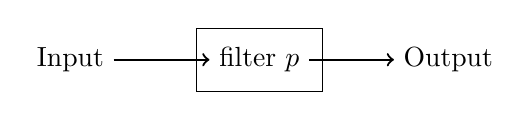
\begin{tikzpicture}[scale=0.8]
      \draw (2, 0) rectangle (4, 1) node (filter) [pos=.5] {filter $p$};
      \draw (0, .5) node (in) {Input}
            (6, .5) node (out) {Output};
      \draw[thick, ->] (in) edge (filter)
                       (filter) edge (out);
      \end{tikzpicture} \\
   \caption{Input: $[x_1, x_2, ..., x_n]$, Output: $[x_1', x_2', ..., x_m']$. and $\forall x_i' \Rightarrow p(x_i')$.}
   \label{fig:filter}
\end{figure}

We can define it in ZF expression:

\be
filter(P, X) = [x_i | x_i \in X, p(x_i)]
\ee

Different from $find$, when there is no element satisfies the predicate, $filter$ returns the empty list. It scans to examine every element one by one:

\be
\begin{array}{rcl}
filter(p,\ \nil) & = & \nil \\
filter(p,\ x:xs) & = & \begin{cases}
  p(x): & x : filter(p, xs) \\
  otherwise: & filter(p, xs) \\
  \end{cases}
\end{array}
\ee

This definition builds the result from right to left. For iterative implementation, if build the result with $append$, it will degrade to $O(n^2)$.

\begin{algorithmic}[1]
\Function{Filter}{$p, L$}
  \State $L' \gets$ NIL
  \While{$L \neq$ NIL}
    \If{$p$(\Call{First}{$L$})}
      \State $L' \gets$ \textproc{Append}($L'$, \Call{First}{$L$}) \Comment{Linear time}
    \EndIf
    \State $L \gets$ \Call{Rest}{$L$}
  \EndWhile
\EndFunction
\end{algorithmic}

The right way is to use $cons$ instead, however, it builds the result in the reversed order. We can further reverse it within linear time (see the exercise). The nature to build result from right indicates that we can define filter in $foldr$. We need define a function $f$ to test an element against the predicate, if OK, prepend to the result:

\be
f(x, A) = \begin{cases}
  p(x): & x : A \\
  otherwise: & A \\
  \end{cases}
\ee

We also need pass the predicate $p$ to $f$. There are actually 3 parameters as $f(p, x, A)$. Filter is defined in $foldr$ with a Curried form of $f$:

\be
filter(p) = foldr((x, A) \mapsto f(p, x, A), \nil)
\ee

We can further simplify it (called $\eta$-conversion\cite{slpj-book-1987}) as:

\be
filter(p) = foldr(f(p), \nil)
\ee

Filter is also a generic concept not only limit to list. We can apply a predicate on any traversable structures to extract the result.

\subsection{Match}
\index{List!matching} \index{List!prefix}
\index{List!suffix} \index{List!infix}

Match is to find a pattern among some structure. Even if we limit to list and string, there are still too many things to cover. We have dedicated chapters about string matching. This section deals with the problem, that given a list $A$, and test if it exits in another list $B$. There are two special cases: to test if $A$ is prefix or suffix of $B$. The $span$ algorithm in (\ref{eq:span}) actually finds a prefix under a certain condition. We can do similar things: to compare each element between $A$ and $B$ from left till meet any different one or reach the end of either list. Define $A \subseteq B$ if $A$ is prefix of $B$:

\be
\begin{array}{rcl}
\nil \subseteq B & = & True \\
(a:as) \subseteq \nil & = & False \\
(a:as) \subseteq (b:bs) & = & \begin{cases}
  a \neq b: & False \\
  a = b: & as \subseteq bs \\
  \end{cases}
\end{array}
\ee

Prefix testing takes linear time as it scans the lists. However, we can not do suffix testing in this way because it is hard to start from the aligned right ends, and scan backwards for lists. This is different from array. Alternatively, we can reverse both lists in linear time, hence change the problem to prefix testing:

\be
A \supseteq B = reverse(A) \subseteq reverse(B)
\ee

With $\subseteq$ defined, we can test if a list is the sub-list of another one. We call it infix testing. The idea is to scan the target list, and repeatedly applying the prefix testing:

\be
\begin{array}{rcl}
infix?(a:as,\ \nil) & = & False \\
infix?(A,\ B) & = & \begin{cases}
  A \subseteq B: & True \\
  otherwise: & infix?(A, B') \\
  \end{cases}
\end{array}
\ee

For the edge case that $A$ is empty, we define empty is infix of any list. Because $\nil \subseteq B$ is always true, it gives the right result. It also evaluates $infix?(\nil, \nil)$ correctly. Below is the corresponding iterative implementation:

\begin{algorithmic}[1]
\Function{Is-Infix}{$A, B$}
  \If{$A = $ NIL}
    \State \Return TRUE
  \EndIf
  \State $n \gets |A|$
  \While{$B \neq$ NIL and $n \leq |B|$}
    \If{$A \subseteq B$}
      \State \Return TRUE
    \EndIf
    \State $B \gets$ \Call{Rest}{$B$}
  \EndWhile
  \State \Return FALSE
\EndFunction
\end{algorithmic}

Because prefix testing runs in linear time, and it is called in the loop of scan. This algorithm is bound to $O(nm)$, where $m, n$ are the length of the two lists respectively. It is an interesting problem to improve this `position by position' scan algorithm to linear time, even when we apply it to arrays. Chapter 13 introduces some smart methods, like the Knuth-Morris-Pratt (KMP) algorithm and Boyer-Moore algorithm. Appendix C introduces another method called suffix-tree.

In a symmetric way, we can enumerate all suffixes of $B$, and check if $A$ is prefix of any of them:

\be
infix?(A, B) = \exists S \in \textit{suffixes}(B), A \subseteq S
\ee

This can be implemented with list comprehension as below example Haskell program:

\begin{Haskell}
isInfixOf a b = (not . null) [ s | s <- tails(b), a `isPrefixOf` s]
\end{Haskell}

Where function \texttt{isPrefixOf} does the prefixing testing, \texttt{tails} generates all suffixes of a given list. We left its implementation as an exercise.

\begin{Exercise}
\Question{Implement the linear time existence testing algorithm.}
\Question{Implement the iterative look up algorithm.}
\Question{Implement the linear time filter algorithm through $reverse$.}
\Question{Implement the iterative prefix testing algorithm.}
\Question{Implement the algorithm to enumerate all suffixes of a list.}
\end{Exercise}

\section{zip and unzip}
\index{List!zip} \index{List!unzip}

The assoc list of paired values is often used as a light weighted dictionary for small set of data. It is easier to build assoc list than tree or heap based dictionary, although the look up performance of assoc list is linear instead of logarithm. In the `$n$-lights' puzzle, we build the assoc list as below:

\[
map(i \mapsto (i, 0),\ [1, 2, ..., n])
\]

More often, we need 'zip' two lists to one. We can define a $zip$ function to do that:

\be
\begin{array}{rcl}
zip(A,\ \nil) & = & \nil \\
zip(\nil,\ B) & = & \nil \\
zip(a:as,\ b:bs) & = & (a, b) : zip(as, bs) \\
\end{array}
\ee

This algorithm works even the two lists have different length. The result length equals to the shorter one. We can even use it to zip infinite lists (under lazy evaluation if both are infinite), for example\footnote{In Haskell: \texttt{zip (repeat 0) [1..n]}}:

\[
zip([0, 0, ...], [1, 2, ..., n])
\]

For a list of words, we can index them with numbers as:

\[
zip([1, 2, ...], [a, an, another, ...])
\]

$zip$ build the result from right. We can also define it with $foldr$. It is bound to $O(m)$ time, where $m$ is the length of the shorter list. When implement the iterative $zip$, the performance will drop to quadratic if using $append$, unless with the reference to the tail position.

\begin{algorithmic}[1]
\Function{Zip}{$A, B$}
  \State $C \gets$ NIL
  \While{$A \neq$ NIL and $B \neq$ NIL}
    \State $C \gets $ \textproc{Append}(C, (\Call{First}{$A$}, \Call{First}{$B$})) \Comment{Linear time}
    \State $A \gets$ \Call{Rest}{$A$}
    \State $B \gets$ \Call{Rest}{$B$}
  \EndWhile
  \State \Return $C$
\EndFunction
\end{algorithmic}

To avoid $append$, we can use 'cons' then reverse the result. However, it can not deal with two infinite lists. In imperative settings, we can also re-use $A$ to store the result (treat it as transform a list of elements to a list of pairs).

We can extend to $zip$ multiple lists to one. Some programming libraries provide, \texttt{zip}, \texttt{zip3}, \texttt{zip4}, ..., till \texttt{zip7}. Sometimes, we don't want to build a list of pairs, but apply a combinator function. For example, given a list of unit prices $[1.00, 0.80, 10.05, ...]$ for fruits: apple, orange, banana, ... When customer has a list of quantities, like $[3, 1, 0, ...]$, means this customer, buys 3 apples, 1 orange, 0 banana, ... Below program generates a payment list:

\[
\begin{array}{rcl}
pays(U,\ \nil) & = & \nil \\
pays(\nil,\ Q) & = & \nil \\
pays(u:us,\ q:qs) & = & (u \cdot q) : pays(us, qs) \\
\end{array}
\]

It is same as the $zip$ function except uses multiply but not 'cons' to combine elements. We can abstract the combinator as a function $f$, and pass it to $zip$ to build a generic algorithm:

\be
\begin{array}{rcl}
zipWith(f, A,\ \nil) & = & \nil \\
zipWith(f, \nil,\ B) & = & \nil \\
zipWith(f, a:as,\ b:bs) & = & f(a, b) : zipWith(f, as, bs) \\
\end{array}
\ee

Here is an example that defines the inner-product (or dot-product)\cite{wiki-dot-product} through $zipWith$:

\be
A \cdot B = sum(zipWith(\cdot, A, B))
\ee

$unzip$ is the inverse operation of $zip$. It converts a list of pairs to two separated lists. Below is its definition with $foldr$ in Curried form:

\be
unzip = foldr((a, b), (A, B) \mapsto (a : A, b : B), (\nil, \nil))
\ee

We fold from a pair of empty lists, break $a, b$ from the pairs and prepend them to the two intermediate lists respectively. We can also use $fst$ and $snd$ explicitly as:

\[
(p, P) \mapsto (fst(p) : fst(P), snd(p) : snd(P))
\]

For the fruits example, suppose the unit price is stored in a assoc list: $U = [(apple, 1.00), (orange, 0.80), (banana, 10.05), ...]$ for lookup, for example $lookup(melon, U)$. The purchase quantity is a assoc list: $Q = [(apple, 3), (orange, 1), (banana, 0), ...]$. How to calculate the total payment? The straight forward way is to extract the unit price and the quantity lists, then compute their inner-product:

\be
pay = sum(zipWith(\cdot, snd(unzip(U)), snd(unzip(Q))))
\ee

$zip$ and $unzip$ are generic. We can expand to $zip$ two trees, where the nodes contain paired elements from both. When traverse a collection of elements, we can also use the generic $zip$ and $unzip$ to track the path, this is a method to mimic the `parent' reference in imperative implementation (last chapter of \cite{learn-haskell}).

\begin{Exercise}
\Question{Design the iota ($I$) algorithm for below usages:
  \begin{itemize}
  \item $iota(..., n) = [1, 2, 3, ..., n]$;
  \item $iota(m, n) = [m, m + 1, m + 2, ..., n]$, where $m \leq n$;
  \item $iota(m, m+a, ..., n) = [m, m + a, m + 2a, ..., n]$;
  \item $iota(m, m, ...) = repeat(m) = [m, m, m, ...]$;
  \item $iota(m, ...) = [m, m + 1, m + 2, ... ]$.
  \end{itemize}
  The last two cases are about infinite list. One possible implementation is through streaming and lazy evaluation (\cite{SICP} and \cite{learn-haskell}).}

\Question{Implement the linear time imperative $zip$ algorithm}

\Question{Define $zip$ with $foldr$.}

\Question{For the fruits example, suppose the quantity assoc list only contains the items with none-zero quantity. i.e. instead of $Q = [(apple, 3), (banana, 0), (orange, 1), ...]$, but $Q = [(apple, 3), (orange, 1), ...]$, because customer does not buy banana. Design a program to calculate the total payment.}

\end{Exercise}

\section{Further reading}
List is the fundamental thing to build more complex data structures and algorithms particularly in functional settings. We introduced elementary algorithms to construct, access, update, and transform list; how to search, filter data, and compute atop list. Although most programming environments provide pre-defined tools and libraries to support list, we should not simply treat them as black-boxes. Rabhi and Lapalme introduce many functional algorithms about list in \cite{algo-fp}. Haskell library provides detailed documentation about basic list algorithms. There are materials provide good examples of folding, especially in \cite{fp-pearls}. It also introduces about the {\em fold fusion law}.

\begin{Exercise}

\Question{Design algorithm to remove the duplicated elements in a list. For imperative implementation, the elements should be removed in-place. The original element order should be maintained. What is the complexity of this algorithm? How to simplify it with additional data structure?}

\Question{List can represent decimal non-negative integer. For example 1024 as list is $4 \rightarrow 2 \rightarrow 0 \rightarrow 1$. Generally, $n = d_m...d_2d_1$ can be represented as
$d_1 \rightarrow d_2 \rightarrow ... \rightarrow d_m$. Given two numbers $a$, $b$ in list form. Realize arithmetic operations such as add and subtraction.}

\Question{In imperative settings, a circular linked-list is corrupted, that some node points back to previous one, as shown in figure \ref{fig:circular-list}. When traverse, it falls into infinite loops. Design an algorithm to detect if a list is circular. On top of that, improve it to find the node where loop starts (the node being pointed by two precedents).}

\end{Exercise}

\begin{figure}[htbp]
\centering
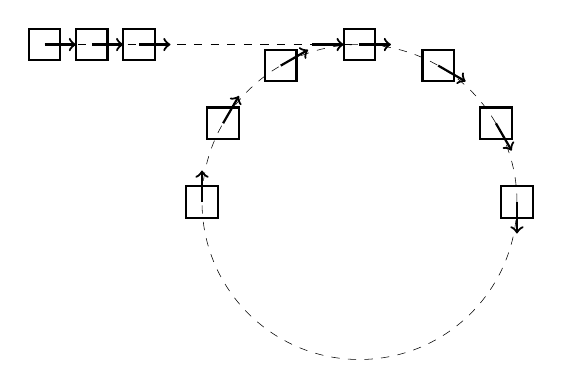
\begin{tikzpicture}[scale=2]
  % trace
  \draw[dashed, very thin] (-2cm, 1cm) -- (0, 1cm);
  \draw[dashed, very thin] (0,0) circle [radius=1cm];

  % leading nodes
  \foreach \x in {-2, -1.7, ..., -1.4} {
    \draw[thick] (\x cm, 1cm) +(-0.1, -0.1) rectangle ++(0.1, 0.1);
    \draw[thick, ->] (\x cm, 1cm) -- +(0.2, 0);
  }

  % cricular starting points
  \draw[thick, ->] (-0.3cm, 1cm) -- (-0.1cm, 1cm);

  % circular nodes
  \foreach \deg/\rot in {90/0, 60/-30, 30/-60, 0/-90, 180/90, 150/60, 120/30} {
    \draw[thick] (\deg : 1cm) +(-0.1, -0.1) rectangle ++(0.1, 0.1);
    \draw[thick, ->] (\deg : 1cm) -- +(\rot : 0.2);
  }
\end{tikzpicture}
\caption{A circular linked-list}
\label{fig:circular-list}
\end{figure}

\begin{thebibliography}{99}

\bibitem{fp-pearls}
Richard Bird. ``Pearls of Functional Algorithm Design''. Cambridge University Press; 1 edition (November 1, 2010). ISBN: 978-0521513388

\bibitem{slpj-book-1987}
Simon L. Peyton Jones. ``The Implementation of Functional Programming Languages''. Prentice-Hall International Series in Computer Since. Prentice Hall (May 1987). ISBN: 978-0134533339

\bibitem{moderncxx}
Andrei Alexandrescu. ``Modern C++ design: Generic Programming and Design Patterns Applied''. Addison Wesley February 01, 2001, ISBN 0-201-70431-5

\bibitem{mittype}
Benjamin C. Pierce. ``Types and Programming Languages''. The MIT Press, 2002. ISBN:0262162091

\bibitem{unplugged}
Xinyu LIU. ``Isomorphism -- mathematics of programming''. 2020. \url{https://github.com/liuxinyu95/unplugged}

\bibitem{SICP}
Harold Abelson, Gerald Jay Sussman, Julie Sussman. ``Structure and Interpretation of Computer Programs, 2nd Edition''. MIT Press, 1996, ISBN 0-262-51087-1

\bibitem{okasaki-book}
Chris Okasaki. ``Purely Functional Data Structures''. Cambridge university press, (July 1, 1999), ISBN-13: 978-0521663502

\bibitem{algo-fp}
Fethi Rabhi, Guy Lapalme. ``Algorithms: a functional programming approach''. Second edition. Addison-Wesley, 1999. ISBN: 0201-59604-0

\bibitem{slpj-book-1987}
Simon Peyton Jones. ``The Implementation of functional programming languages''. Prentice-Hall International, 1987. ISBN: 0-13-453333-X

\bibitem{learn-haskell}
Miran Lipovaca. ``Learn You a Haskell for Great Good! A Beginner's Guide''. No Starch Press; 1 edition April 2011, 400 pp. ISBN: 978-1-59327-283-8

\bibitem{erlang}
Joe Armstrong. ``Programming Erlang: Software for a Concurrent World''. Pragmatic Bookshelf; 1 edition (July 18, 2007). ISBN-13: 978-1934356005

\bibitem{wiki-tail-call}
Wikipedia. ``Tail call''. https://en.wikipedia.org/wiki/Tail\_call

\bibitem{sgi-stl-transform}
SGI. ``transform''. http://www.sgi.com/tech/stl/transform.html

\bibitem{poj-drunk-jailer}
ACM/ICPC. ``The drunk jailer.'' Peking University judge online for ACM/ICPC. http://poj.org/problem?id=1218.

\bibitem{Haskell-wiki}
Haskell wiki. ``Haskell programming tips''. 4.4 Choose the appropriate fold. http://www.haskell.org/haskellwiki/Haskell\_programming\_tips

\bibitem{wiki-dot-product}
Wikipedia. ``Dot product''. http://en.wikipedia.org/wiki/Dot\_product

\end{thebibliography}

\ifx\wholebook\relax \else
\end{document}
\fi
